\section{Arquitetura do Sistema de Software} % (fold)
\label{sub:arquitetura}

Em relação a arquitetura do sistema, a mesma foi definida em módulos, contemplando 5 módulos distribuídos. A comunicação entre os principais módulos é feita a partir da utilização de \textit{sockets} por conexão TCP. De modo geral, a arquitetura pode ser representada pela Figura \ref{img:arquitetura}.

\begin{figure}[H]
	\centering
	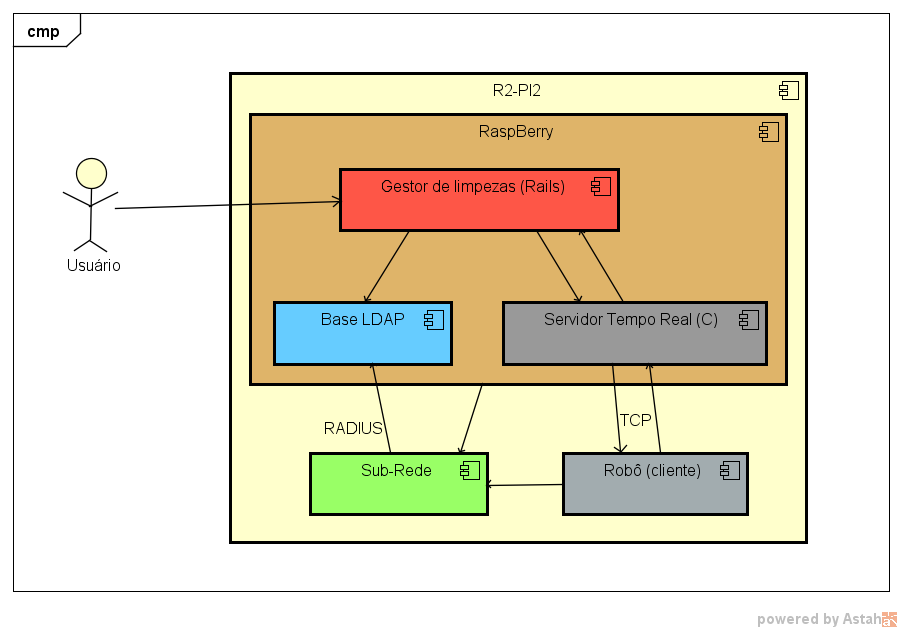
\includegraphics[scale=0.7]{figuras/diagrama_arquitetural.png}
	\caption{Diagrama arquitetural do sistema R2-PI2.}
	\label{img:arquitetura}
\end{figure}

O \textit{Servidor Tempo Real} gerencia diversas \textit{threads} para processar e instruir informações ao robô. O escalonamento destas \textit{threads} segue o padrão de sistemas em tempo real, a partir da configuração do \textit{patch RT\_Preempt} no Kernel utilizado no servidor. Desse modo, o tempo de resposta a requisições advindas do robô é otimizado, buscado evitar falhas de controle relacionadas ao atraso do sistema.

A comunicação entre Robô e Servidor Tempo Real segue uma arquitetura cliente-servidor, onde o cliente e o servidor acabam trocando de papéis em determinadas ocasiões. Em alguns instantes o robô fará requisições ao servidor, que lhe retorna uma resposta, já em outros instantes o servidor fará requisições ao robô, obtendo também uma resposta. 

O principal motivo da escolha desta arquitetura se refere ao poder de processamento presente no servidor, em relação ao processamento encontrado no robô (ATMega). Como o sistema é caracterizado como um sistema de tempo real, necessitou-se da utilização deste mecanismo de processamento.

Como interface do sistema para o cliente, foi desenvolvido o sistema Gestor de Limpezas, em rails. Este sistema faz comunicação com o Sistema Tempo Real e a base de registro de usuários (LDAP). Neste sistema é possível agendar limpezas, iniciar e parar uma limpeza e análisar \textit{status} de limpeza. A comunicação entre os dois sistemas é feita a partir de sockets locais, já que os dois serão executados na mesma máquina (raspberry pi).